\documentclass{beamer}

\usepackage{graphicx,url}
\usepackage[brazil]{babel}  \usepackage[utf8]{inputenc}
\usepackage{subfigure}

\usetheme{Warsaw}
\title[Compart. Arquiv. em Storage de Alta Disponibilidade]{Compartilhamento de Arquivos\\ em Storage de Alta Disponibilidade}
\author{Leonardo Antônio dos Santos}
\institute{Faculdades Integradas do Brasil - UniBrasil}
%Orientador: ???\\
%Co-orientador: Pedro Eugênio Rocha
\date{Curitiba/2012}
\begin{document}


\begin{frame}
\titlepage
\end{frame}


\begin{frame}{Orientação}
\begin{itemize}
\item \textbf{Orientador:} ???
\item \textbf{Co-orientador:} Msc. Pedro Eugênio Rocha
\end{itemize}
\end{frame}


\begin{frame}{Introdução}
\begin{itemize}
\item \textbf{OBJETO DE ESTUDO:} Sistemas Web, Protocolos de Rede, Sistemas Distribuídos.  	\\
\item \textbf{CONTEXTO:} Compartilhamento de arquivos em storage de alta disponibilidade para a infraestrutura de TI da UniBrasil via Intranet, em SAN (Storage Area Network) e através do Protocolo AoE (ATA over Ethernet). \\
\item \textbf{O QUE SE DISCUTE?} Um sistema Web que faz uso de um protocolo de código aberto - AoE - para disponibilização de espaço em disco de forma distribuída, com alta disponibilidade e performance. Podendo ainda a infraestrutura gerada pela implementação deste protocolo ser utilizada para qualquer outra finalidade de armazenamento. 
\end{itemize}
\end{frame}


\begin{frame}{Problema de Pesquisa}
\begin{itemize}[<+->]
\item Inexistência de uma área de armazenamento de dados compartilhada entre todo o corpo docente e discente da UniBrasil.
\item Alto custo nas tecnologias de armazenamento de dados para compartilhamento de alta disponibilidade.
\end{itemize}
\end{frame}


\begin{frame}{Objetivo Geral}
Tornar possível o uso de um protocolo e uma aplicação web que, integrados, permitam compartilhar arquivos com alta disponibilidade na intranet da UniBrasil e na internet.
\end{frame}


\begin{frame}{Objetivos Específicos}
\begin{itemize}
\item Estudar sobre protocolos de rede, alta disponibilidade de dados, analise de performance e aplicações web;
\item Avaliar tecnologias paralelas que já encontram-se em uso no mercado;
\item Implementar um protocolo adaptando-o a uma infraestrutura capaz de compartilhar dados pela intranet e pela internet via web de forma distribuída;
\item Desenvolver sistema web que facilite o uso desta tecnologia ao usuário final;
\end{itemize}
\end{frame}


\begin{frame}{Justificativa}
\begin{itemize}
\item O compartilhamento de arquivos, apesar de ser simples utilizando as ferramentas conhecidas, torna-se muito custoso quando se busca implementar grandes áreas de armazenamento de dados, principalmente se forem distribuídos e com alta disponibilidade. Isto acontece devido ao fato desta implementação ser possível somente com a compra de equipamentos especializados para este fim.
\item O protocolo AoE aparece com a finalidade de resolver problemas de compartilhamento de arquivos, só que a um baixo custo de tecnologia, se comparado a protocolos para \textit{filesystems} (sistemas de arquivos) distribuídos.
\item Uma implementação completa deste protocolo juntamente com uma ferramenta Web que facilitará e orquestrará o seu uso.
\end{itemize}
\end{frame}


\begin{frame}{Metodologia da Pesquisa}
\begin{itemize}
\item \textbf{Natureza da pesquisa:} Redes de Computadores e Sistemas Distribuídos (Protocolos de Comunicação, Arquitetura de \textit{Clusters} e Servidores, Sistemas Distribuídos, Alta Disponibilidade).
\item \textbf{Tipo de pesquisa:} Aplicada e Bibliográfica.
\item \textbf{Levantamento de requisitos:} Levantamento das necessidades de compartilhamento de arquivos utilizando-se de mecanismos como entrevistas e análise dos sistemas existentes.
\end{itemize}
\end{frame}

\begin{frame}{Revisão de Literatura}
\begin{itemize}
	\item COMPARTILHAMENTO DE ARQUIVOS
		\begin{itemize}
		\item Compartilhamento NAS (\textit{Network Attached Storage})
		\item Compartilhamento SAN (\textit{Storage Area Network})
		\item NAS vs. SAN
		\end{itemize}
	\item PROTOCOLOS PARA COMPARTILHAMENTO DE DISCOS
		\begin{itemize}
		\item ATA Over Ethernet (AoE)
		\item iSCSI
		\item Análise de Desempenho
		\end{itemize}
	\item ALTA DISPONIBILIDADE
		\begin{itemize}
		\item RAID
		\end{itemize}
	\item SOLUÇÃO PROPOSTA
		\begin{itemize}
		\item Soluções Tecnológicas Semelhantes
		\item Arquitetura da Solução
		\end{itemize}
\end{itemize}
\end{frame}

\begin{frame}{Compartilhamento de Arquivos / NAS}
\begin{itemize}
	\item Compartilha \textbf{Arquivos}
	\item \textbf{Não possui} uma rede separada para esta finalidade.
\end{itemize}
\begin{figure}[h]
\centering
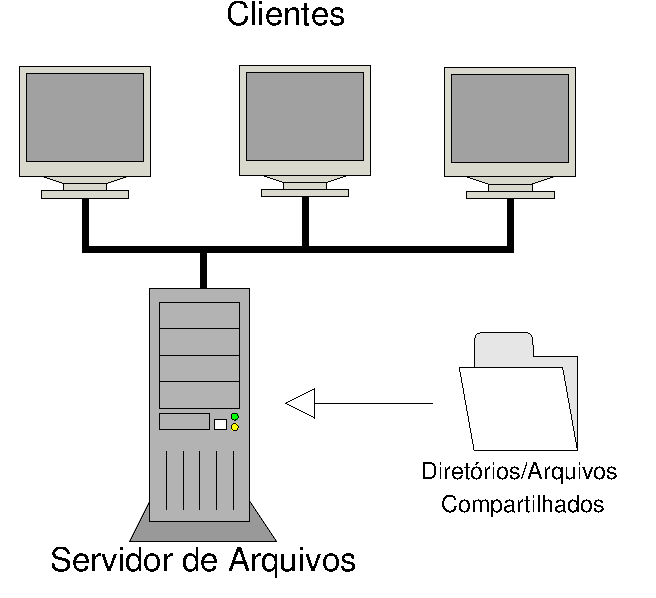
\includegraphics[width=5cm]{img/nas.pdf} 
 \label{fig-nas}
\end{figure}
\end{frame}

\begin{frame}{Compartilhamento de Arquivos / NAS}
\begin{itemize}
	\item Compartilha \textbf{Arquivos}
	\item \textbf{Não possui} uma rede separada para esta finalidade.
\end{itemize}
\begin{figure}[h]
\centering
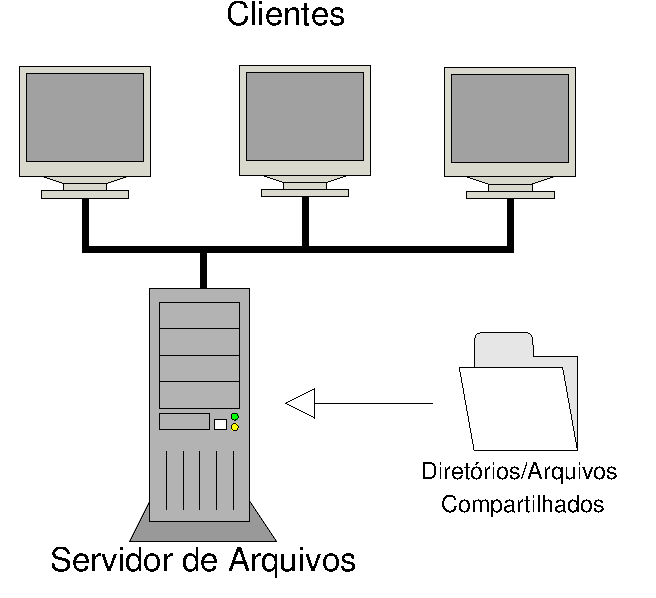
\includegraphics[width=5cm]{img/nas.pdf} 
 \label{fig-nas}
\end{figure}
\end{frame}


\begin{frame}{Compartilhamento de Arquivos / SAN}
\begin{itemize}
	\item Compartilha \textbf{Discos}
	\item \textbf{Possui} uma rede separada para esta finalidade.
\end{itemize}
\begin{figure}[h]
	\centering
	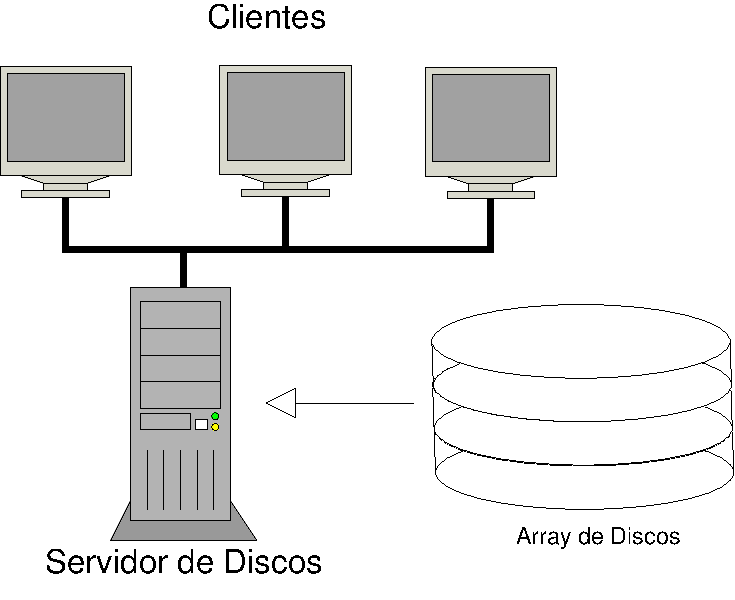
\includegraphics[width=5cm]{img/san.pdf} 
	 \label{fig-nas}
\end{figure}
\end{frame}


\begin{frame}{NAS vs. SAN}
\begin{itemize}[<+->]
	\item A solução SAN torna-se mais viável para funcionamento de toda a infraestrutura de alta disponibilidade nos padrões atuais, visto que tecnologias de redundância de dados como RAID não funcionam sobre arquivos, mas sobre disco.
	\item Toda a lógica de redundância fica transparente ao usuário final.
	\item As demandas de virtualização têm tornado o SAN mais importante.
\end{itemize}
\end{frame}


\begin{frame}{Protocolos para Compatilhamento SAN}
\begin{itemize}
	\item \textbf{AoE:} 
	\begin{itemize}
		\item Funciona na camada Ethernet (2) do modelo TCP/IP.
		\item Não faz roteamento para a internet (pode ser feito através de Middleware).
	\end{itemize}
	\item \textbf{iSCSI: } 
	\begin{itemize}
		\item Funciona na camada de Rede (3) do modelo TCP/IP.
		\item Faz roteamento de forma nativa.
	\end{itemize}
\end{itemize}
\begin{figure}[hbtp]
	\centering
	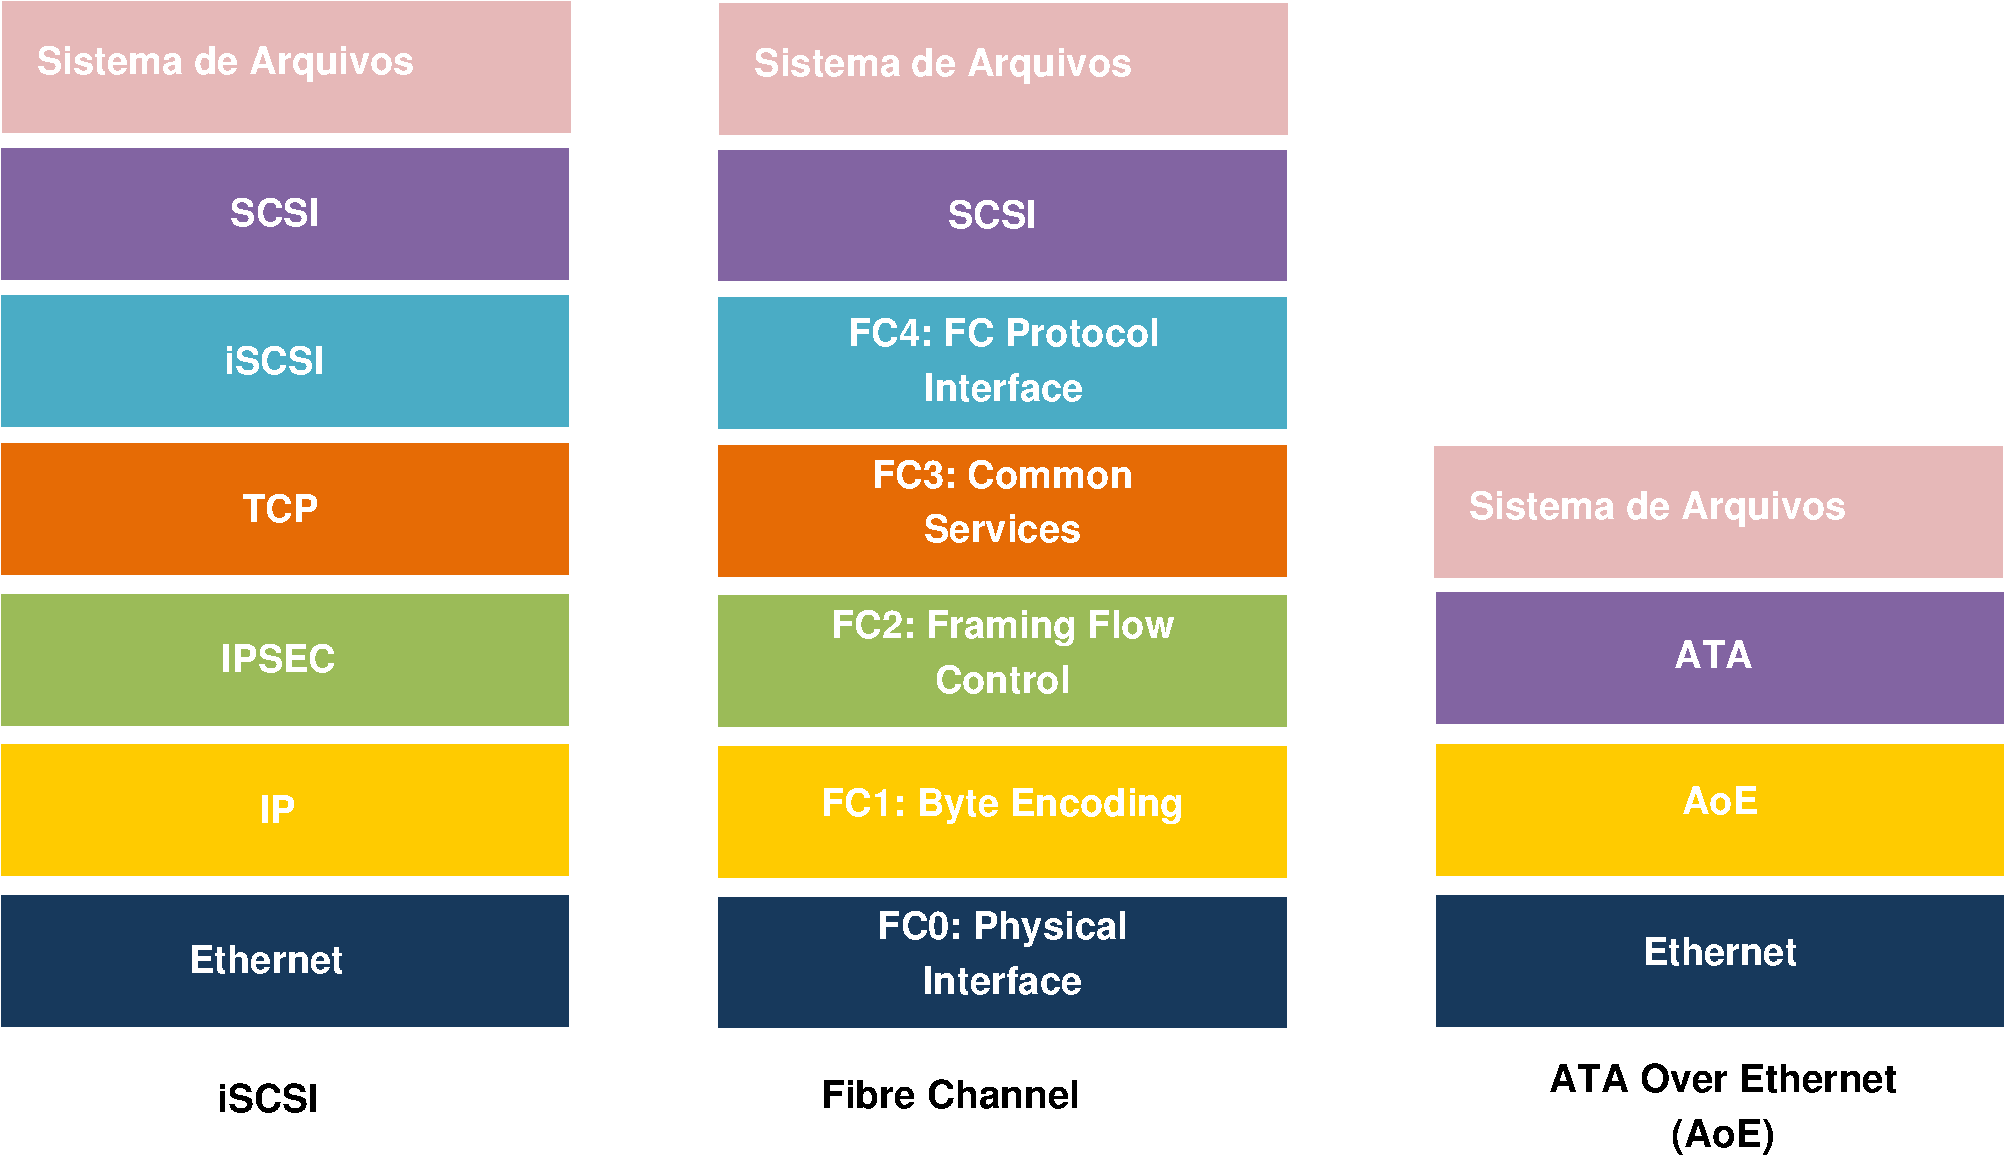
\includegraphics[width=.7\linewidth]{./img/comparativo_camadas}
	\label{fig_comparativo_protocolos}
\end{figure}
\end{frame}


\begin{frame}{Análise de Desempenho - Vazão}
\begin{figure}[ht] 
	\centering
	\subfigure[webserver-throughput][Webserver] {
		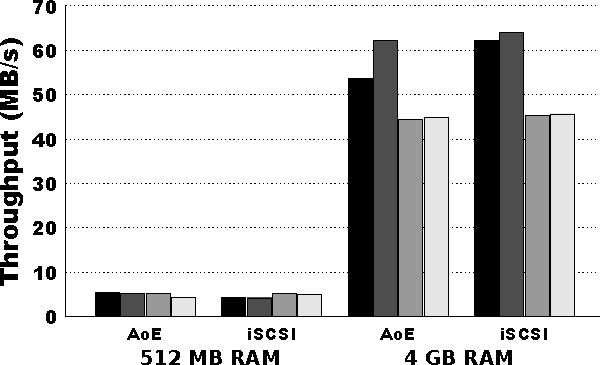
\includegraphics[width=4cm]{img/desempenho/webserver-throughput.pdf} 
		\label{webserver-throughput} 
	}
	\quad
	\subfigure[fileserver-throughput][Fileserver] {
		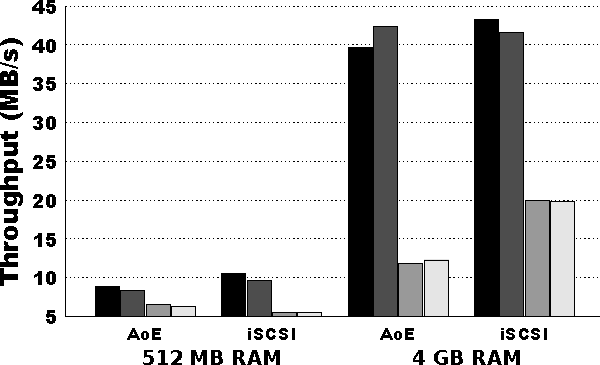
\includegraphics[width=4cm]{img/desempenho/fileserver-throughput.pdf} 
		\label{fileserver-throughput} 
	}
	\quad
	\subfigure[varmail-throughput][Varmail] {
		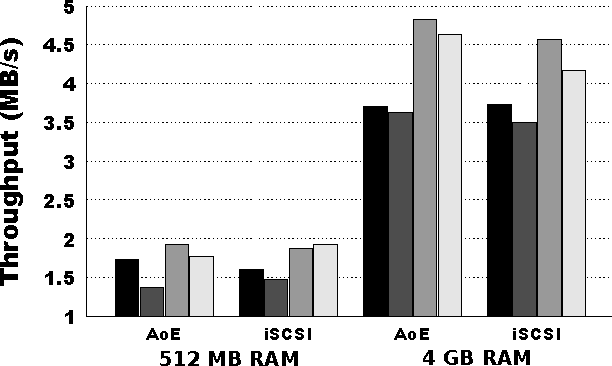
\includegraphics[width=4cm]{img/desempenho/varmail-throughput.pdf} 
		\label{varmail-throughput} 
	}	
	\quad
	\subfigure[oltp-throughput][Oltp] {
		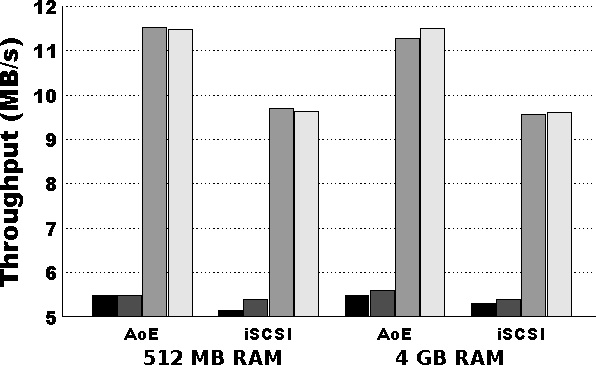
\includegraphics[width=4cm]{img/desempenho/oltp-throughput.pdf} 
		\label{oltp-throughput} 
	}
	\quad
	\subfigure {
		
\includegraphics[width=\linewidth]{img/desempenho/legenda} 
	}
\end{figure}
\end{frame}

\begin{frame}{Análise de Desempenho - CPU}
\begin{figure}[ht] 
	\centering
	\subfigure[webserver-throughput][Webserver] {
		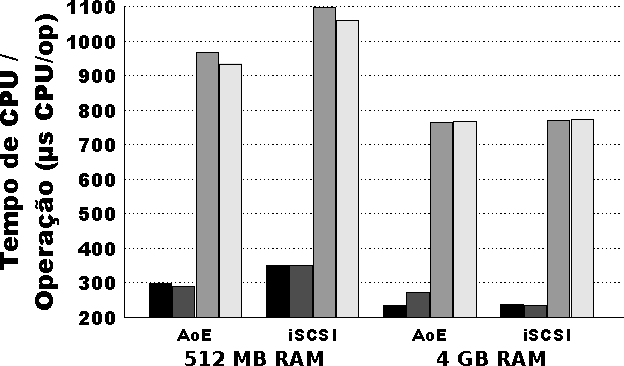
\includegraphics[width=4cm]{img/desempenho/webserver-cpu.pdf} 
	}
	\quad
	\subfigure[fileserver-throughput][Fileserver] {
		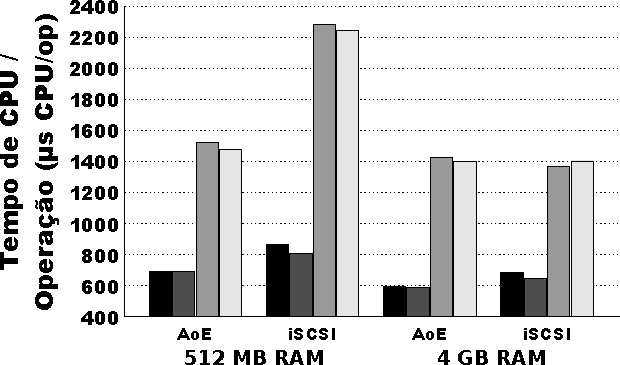
\includegraphics[width=4cm]{img/desempenho/fileserver-cpu.pdf} 
	}
	\quad
	\subfigure[varmail-throughput][Varmail] {
		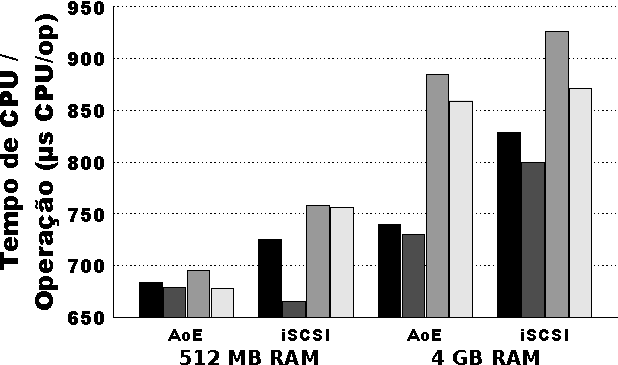
\includegraphics[width=4cm]{img/desempenho/varmail-cpu.pdf} 
	}	
	\quad
	\subfigure[oltp-throughput][Oltp] {
		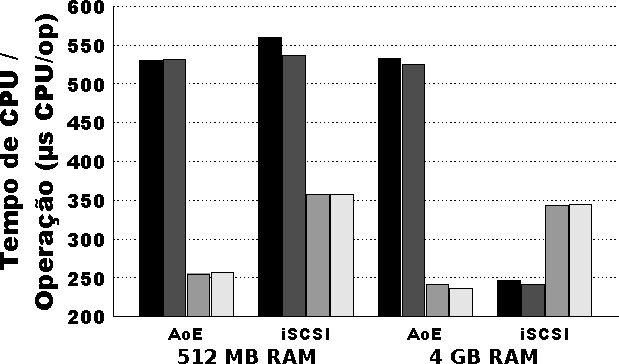
\includegraphics[width=4cm]{img/desempenho/oltp-cpu.pdf} 
	}
	\quad
	\subfigure {
		
\includegraphics[width=\linewidth]{img/desempenho/legenda} 
	}
\end{figure}
\end{frame}

\begin{frame}{Análise de Desempenho - Rede}
\begin{figure}[ht] 
	\centering
	\subfigure[webserver-throughput][Webserver] {
		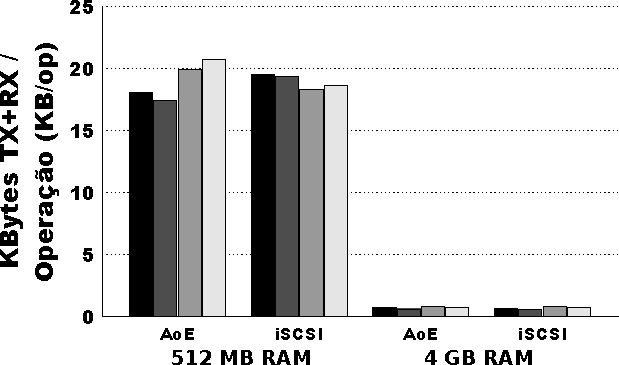
\includegraphics[width=4cm]{img/desempenho/webserver-rede.pdf} 
	}
	\quad
	\subfigure[fileserver-throughput][Fileserver] {
		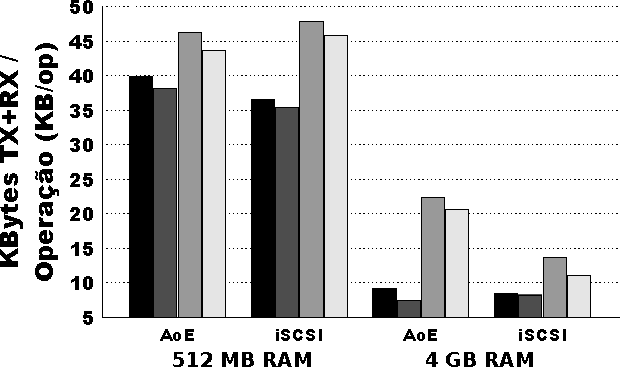
\includegraphics[width=4cm]{img/desempenho/fileserver-rede.pdf} 
	}
	\quad
	\subfigure[varmail-throughput][Varmail] {
		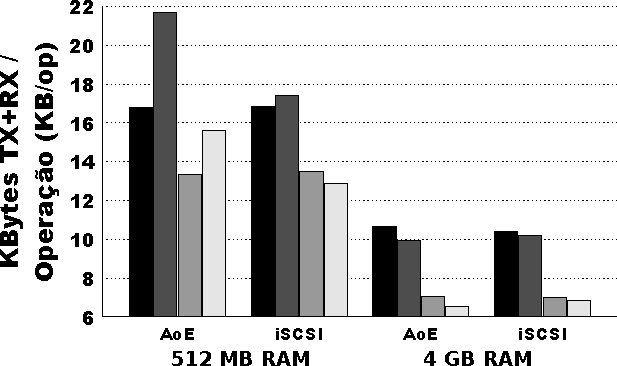
\includegraphics[width=4cm]{img/desempenho/varmail-rede.pdf} 
	}	
	\quad
	\subfigure[oltp-throughput][Oltp] {
		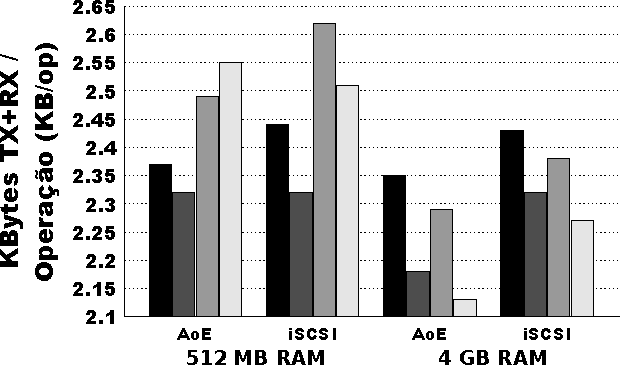
\includegraphics[width=4cm]{img/desempenho/oltp-rede.pdf} 
	}
	\quad
	\subfigure {
		
\includegraphics[width=\linewidth]{img/desempenho/legenda} 
	}
\end{figure}
\end{frame}


\begin{frame}{Publicação de Artigo}
\begin{itemize}
\item \textbf{Data submissão:} 30/04/2012 (segunda-feira).
\item \textbf{Evento:} SEMISH - XXXIX Seminário Integrado de Software e Hardware.
\item \textbf{Local:} Curitiba/PR.
\item \textbf{Foco:} \textit{"Este ano temos interesse particular em computação ubíqua, compreendendo estudos e soluções para serviços e infraestruturas convergentes, cloud computing, virtualização e mobilidade."}
\end{itemize}
\end{frame}


\begin{frame}{Alta Disponibilidade}
\begin{itemize}
	\item RAID
		\begin{itemize}
		\item Stripping
		\item Paridade
		\item Espelhamento
		\item Hot Spare
		\end{itemize}
\end{itemize}
\end{frame}


\begin{frame}{Alta Disponibilidade / RAID}
\begin{figure}[ht]
\subfigure[hc][RAID nível 0]{
 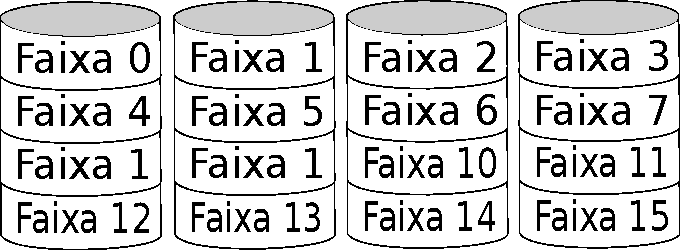
\includegraphics[width=5cm]{img/raid0.pdf} 
 \label{raid0}
}
\subfigure[hc][RAID nível 1]{
 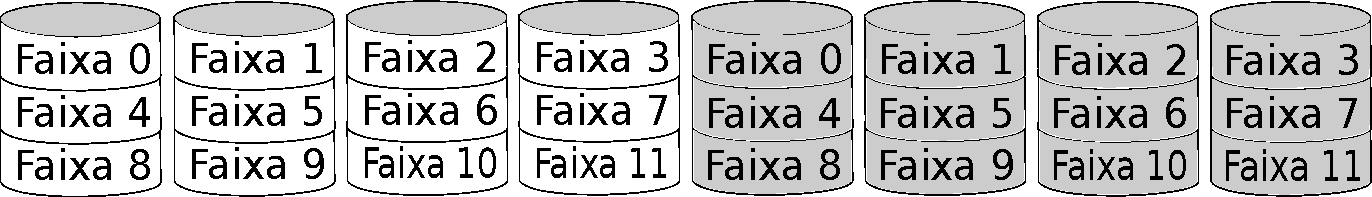
\includegraphics[width=\linewidth]{img/raid1.pdf} 
 \label{raid1}
}
\subfigure[hc][RAID nível 5]{
 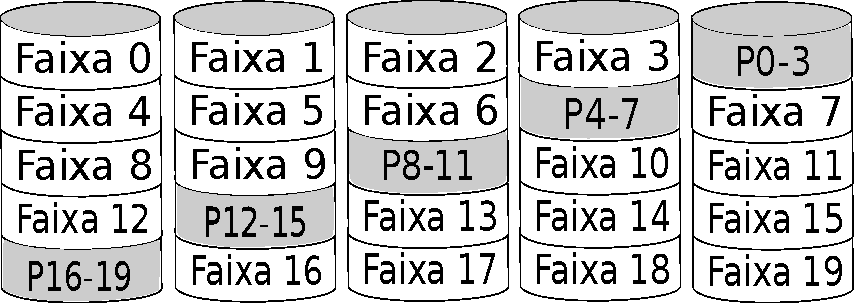
\includegraphics[width=5cm]{img/raid5.pdf} 
 \label{raid5}
}
\end{figure}
\end{frame}


\begin{frame}{Arquitetura da Solução Tecnológica}
\begin{center}
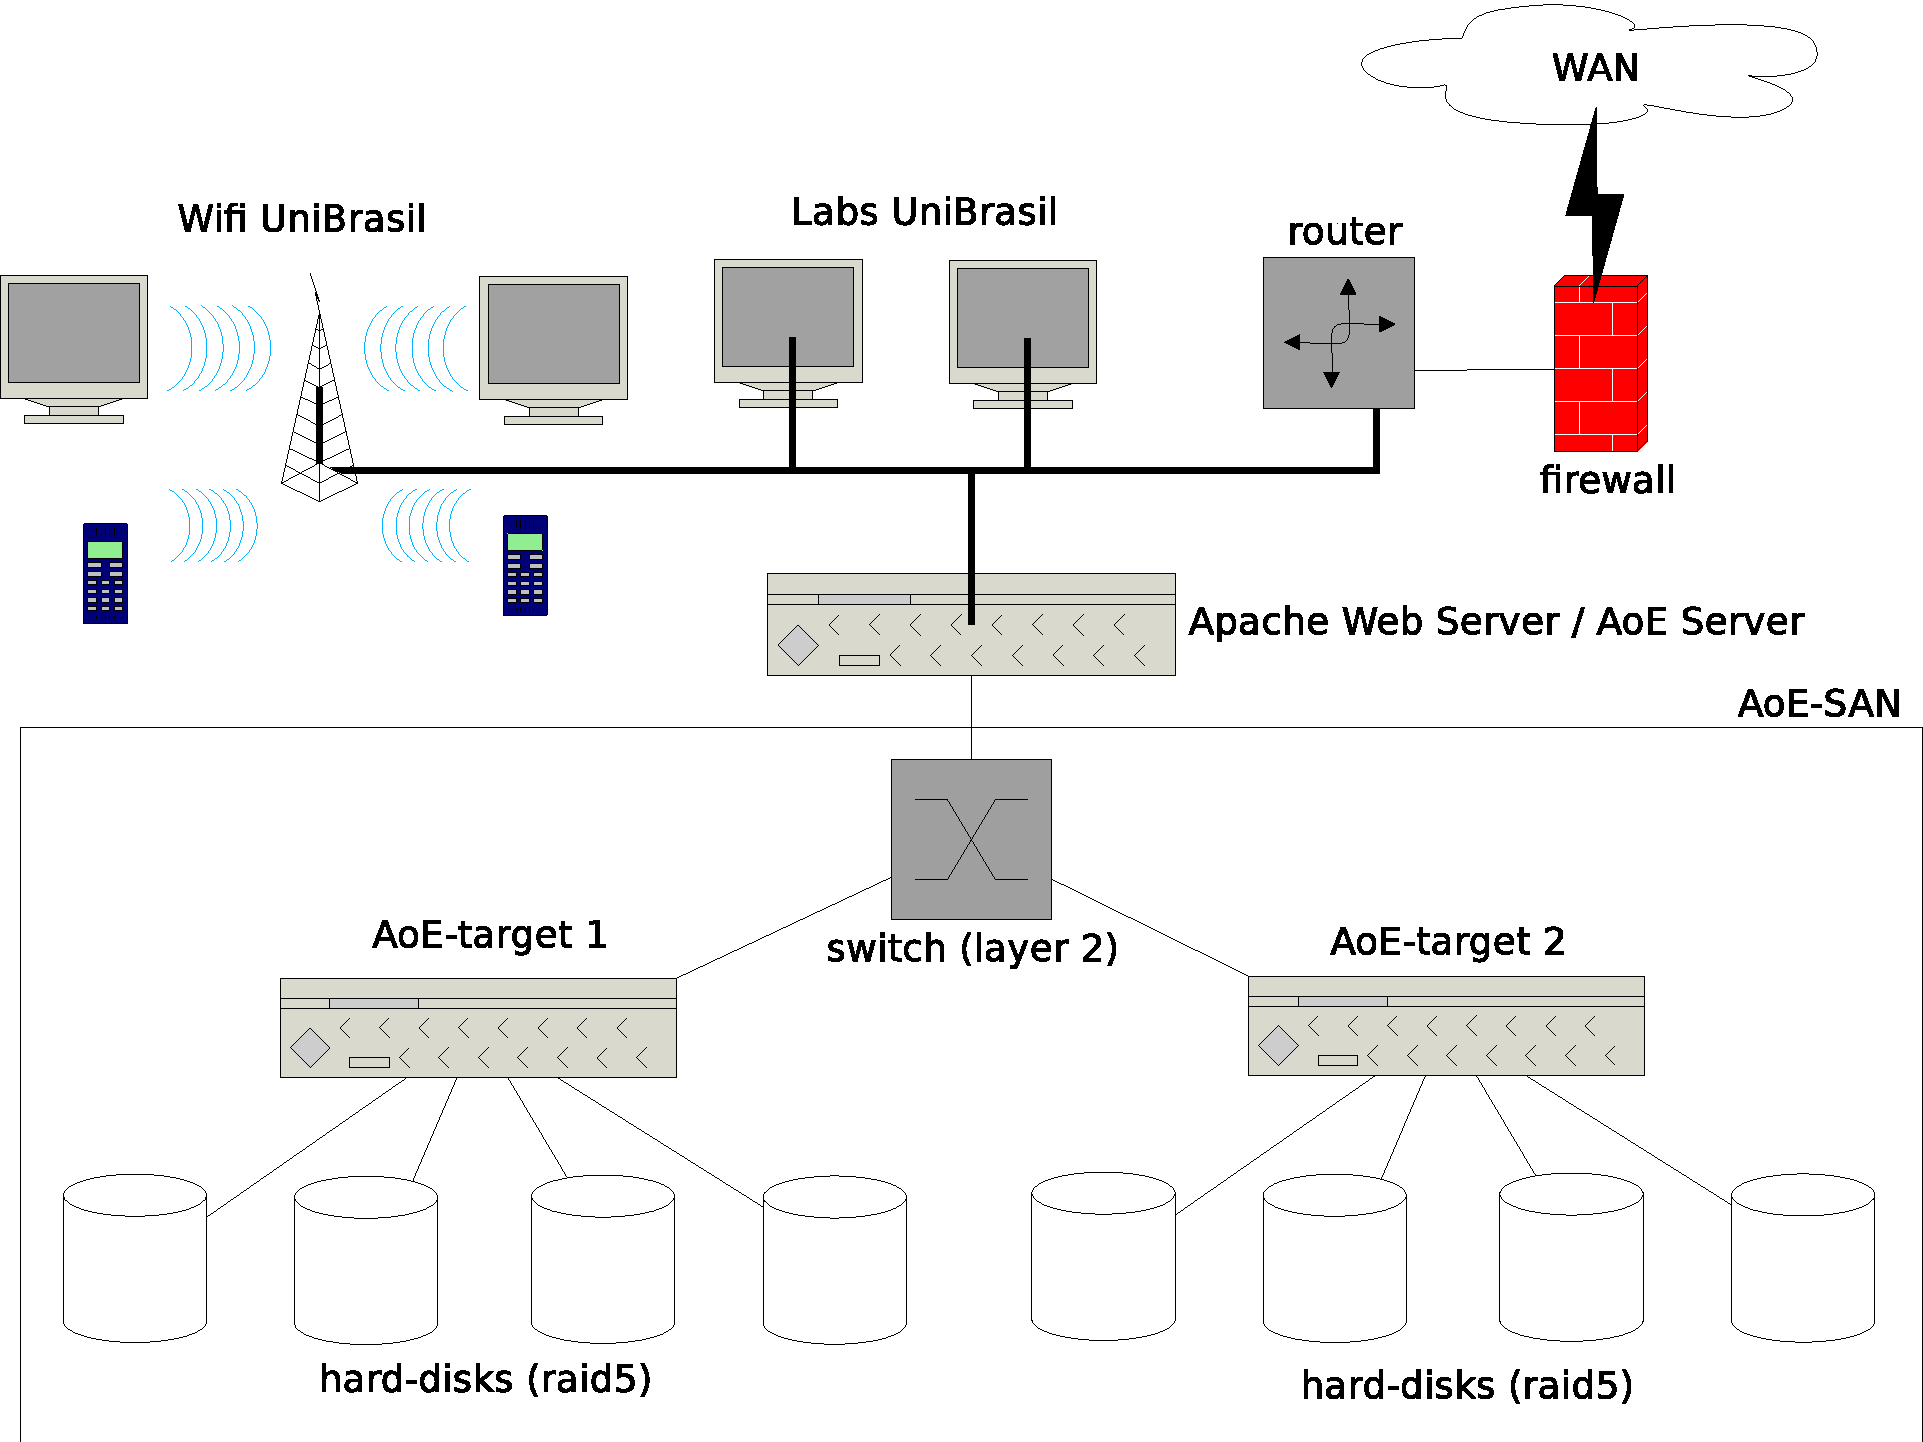
\includegraphics[width=10cm]{./img/arquitetura-solucao}
\end{center}
\end{frame}


\begin{frame}{Cronograma}
\begin{center}
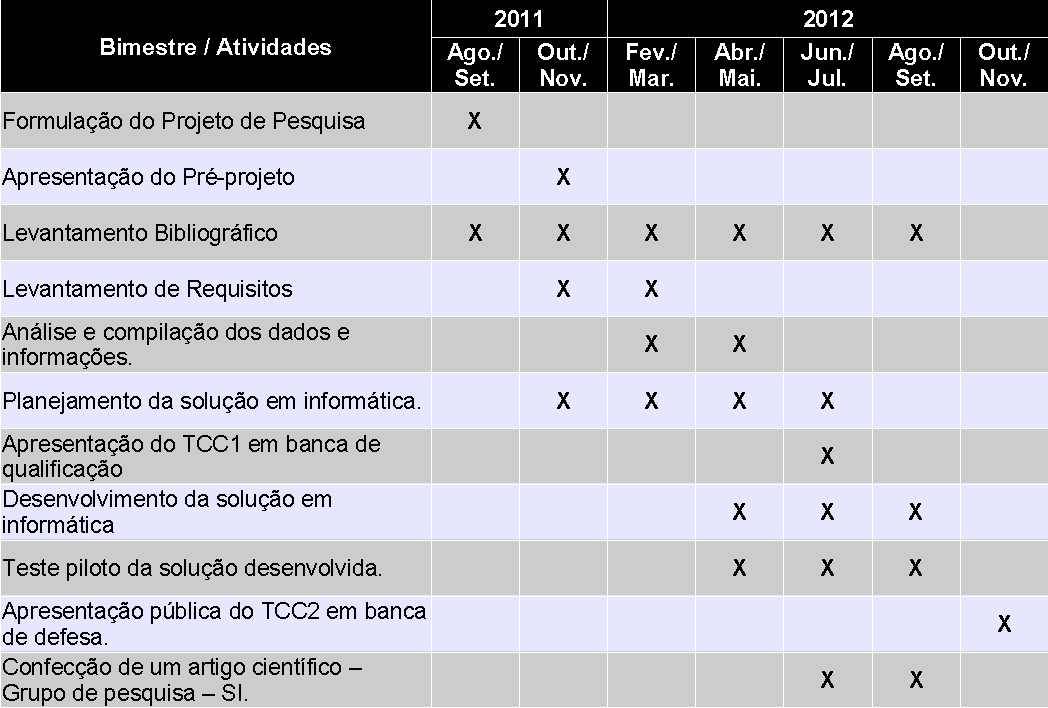
\includegraphics[width=\textwidth]{./img/tab-cronograma}
\end{center}
\end{frame}


\begin{frame}{Tecnologias Utilizadas}
\begin{center}
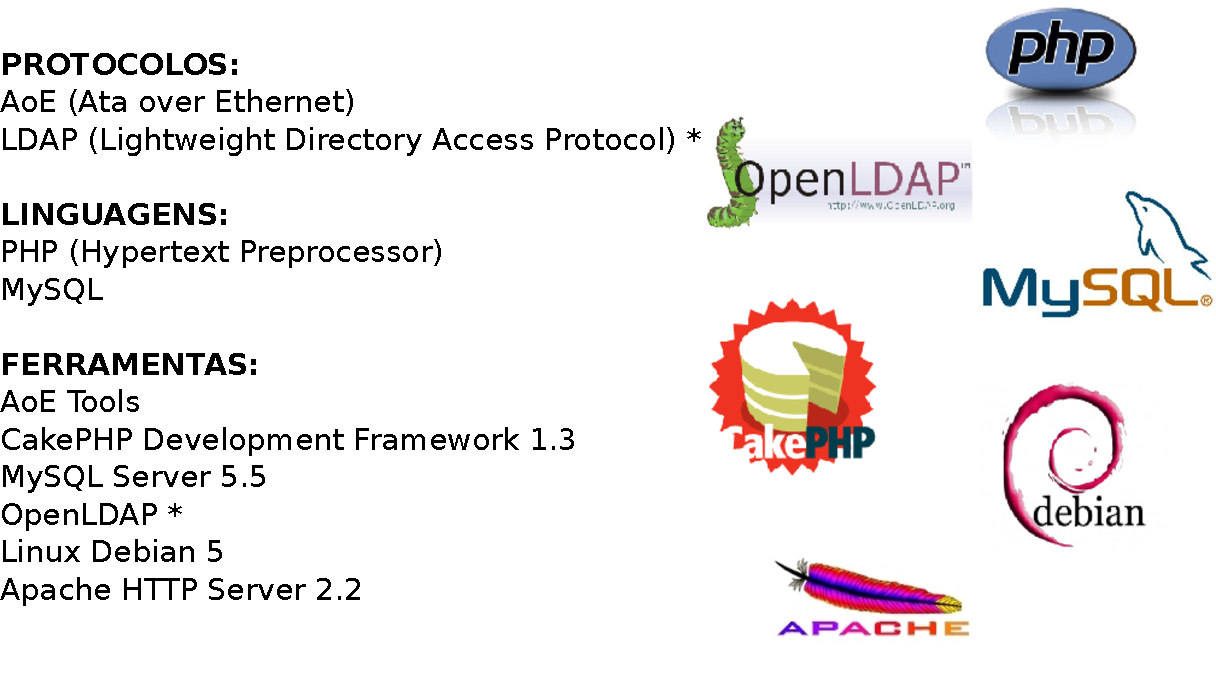
\includegraphics[width=\textwidth]{./work/tecnologias}
\end{center}
\end{frame}


%---------- Referencias ----------
% \bibliographystyle{abnt-alf} % habilita colchetes
\begin{frame}{Bibliografia}
\begin{itemize}
\item 4SHARED.COM - free file sharing and storage. [S.l.]: 4shared.com, 2005. http://www.4shared.com/. Acesso em: 20 set. 2011.
\item AIKEN, S. et al. A performance analysis of the iscsi protocol. In: Mass Storage Systems and Technologies, 2003. (MSST 2003). Proceedings. 20th IEEE/11th NASA Goddard Conference on. [S.l.: s.n.], 2003. p. 123 – 134.
\item CLARK, T. Designing storage area networks: a practical reference for implementing Fibre Channel SANs. Boston, MA, USA: Addison-Wesley Longman Publishing Co., Inc., 1999. ISBN 0-201-61584-3.
\item FASHEH, M. Ocfs2: The oracle clustered file system, version 2. In: Linux Symposium. [S.l.: s.n.], 2006. Maio de 2007: http://oss.oracle.com/projects/ocfs2/dist/documentation/fasheh.pdf.
\item  FUNDAMENTALS of Networked Storage. [S.l.]: vmworld.com/docs/DOC-1374. 
\end{itemize}
\end{frame}

\begin{frame}{Bibliografia}
\begin{itemize}
\item Coraid, Inc, 2008. http://www.HOPKINS, S.; COILE, B. ATA over Ethernet Specification. [S.l.]: The Brantley Coile Company, Inc, 2001. http://support.coraid.com/documents/AoEr11.txt.
\item LANDOWSKI, M.; CURRAN, P. F. Aoe storage protocol over mpls network. In: Proceedings of the 2011 IEEE 27th Symposium on Mass Storage Systems and Technologies. Washington, DC, USA: IEEE Computer Society, 2011. (MSST ’11), p. 1–5. ISBN 978-1-4577-0427-7. Disponível em: <http://dx.doi.org/10.1109/MSST.2011.5937231>.
\item LEWIS, A. LVM HOWTO. [S.l.]: The Linux Documentation Project, 2006. http://www.tldp.org/HOWTO/LVM-HOWTO/.
\item PATTERSON, D. A.; GIBSON, G. A.; KATZ, R. H. A case for redundant arrays of inexpensive disks (raid). In: SIGMOD Conference. [S.l.: s.n.], 1988. p. 109–116.
\item SATRAN, J. et al. Internet Small Computer Systems Interface (iSCSI). IETF, abr. 2004. RFC 3720 (Proposed Standard). (Request for Comments, 3720). Updated by RFCs 3980, 4850, 5048. Disponível em: <http://www.ietf.org/rfc/rfc3720.txt>.
\end{itemize}
\end{frame}

\begin{frame}{Bibliografia}
\begin{itemize}
\item SOURCEFORGE.NET: Find, Create, and Publish Open Source software for free. [S.l.]: 2011 Geeknet, Inc, 2011. http://sourceforge.net/. Acesso em: 20 set. 2011.
\item TANENBAUM, A. S. Sistemas Operacionais Modernos. trad. 3 ed. São Paulo: Pearson, 2010.
\item VAGHANI, S. B. Virtual machine file system. SIGOPS Oper. Syst. Rev., ACM, New York, NY, USA, v. 44, n. 4, p. 57–70, dez. 2010. ISSN 0163-5980. Disponível em: <http://doi.acm.org/10.1145/1899928.1899935>.
\item YOUTUBE - Broadcast Yourself. [S.l.]: 2011 YouTube, LLC, 2011. http://www.
youtube.com/. Acesso em: 20 set. 2011.
\end{itemize}
\end{frame}

\end{document}